\documentclass{BeamerTemplate}

\usepackage{pgfplotstable}
\usepgfplotslibrary{statistics}
\pgfplotsset{compat=1.17}

\title{Chapitre 1 -- La statistique descriptive}
\subtitle{STT-1920 Méthodes statistiques}
\date{}

% ---------------------------------------------------------------------------
% Styles des graphiques
% ---------------------------------------------------------------------------
\pgfplotsset{
  base/.style={
    tick label style={font=\scriptsize}, label style={font=\small},
    title style={font=\small\bfseries},
    yticklabel style={/pgf/number format/fixed, /pgf/number format/precision=3},
    scaled y ticks=false, axis lines*=left,
  },
  % Histogramme des poids des 147 serpents
  histserp/.style={base, width=7.2cm, height=5cm, ymin=0,
    xlabel={Poids (g)}, ylabel={Fréquence}},
  barres/.style={ybar interval, fill=Dominante!60, draw=black},
  % Petits histogrammes (formes de distributions)
  mini/.style={base, width=4.9cm, height=4cm, ymin=0, ytick=\empty,
    axis y line=none, title style={font=\scriptsize\bfseries}},
  % Diagramme en boîte horizontal sans graduation verticale
  boiteh/.style={base, axis y line=none, ytick=\empty, ymin=0.4, ymax=1.6},
  % Boîte « préparée » : boiteprep={min bras}{Q1}{Q2}{Q3}{max bras}
  boiteprep/.style n args={5}{draw=black, fill=Dominante!40, thick,
    boxplot prepared={draw position=1, box extend=0.5,
      lower whisker=#1, lower quartile=#2, median=#3,
      upper quartile=#4, upper whisker=#5}},
}

% Données des histogrammes (tableaux x = borne gauche, y = hauteur)
% Trois formes de distributions (données simulées, n = 200)
\pgfplotstableread[row sep=\\]{
  x y\\ 90 1\\ 95 4\\ 100 12\\ 105 18\\ 110 23\\ 115 40\\ 120 35\\ 125 35\\
  130 17\\ 135 10\\ 140 3\\ 145 2\\ 150 0\\
}\tabsym
\pgfplotstableread[row sep=\\]{
  x y\\ 0 16\\ 1.5 61\\ 3 43\\ 4.5 38\\ 6 11\\ 7.5 11\\ 9 12\\ 10.5 1\\ 12 2\\
  13.5 1\\ 15 2\\ 16.5 1\\ 18 0\\ 19.5 1\\ 21 0\\
}\tabdro
\pgfplotstableread[row sep=\\]{
  x y\\ 30.5 1\\ 31.25 0\\ 32 0\\ 32.75 1\\ 33.5 1\\ 34.25 2\\ 35 5\\ 35.75
  3\\ 36.5 8\\ 37.25 21\\ 38 18\\ 38.75 42\\ 39.5 52\\ 40.25 46\\ 41 0\\
}\tabgau
\pgfplotstableread[row sep=\\]{
  x y\\ 32.5 4\\ 33 5\\ 33.5 16\\ 34 30\\ 34.5 24\\ 35 29\\ 35.5 21\\ 36 11\\
  36.5 5\\ 37 1\\ 37.5 1\\ 38 0\\
}\tabserp

\begin{document}

\begin{frame}[t]
  \titlepage
\end{frame}

%===============================================================================
\section[Introduction]{1.1 Introduction}
%===============================================================================

\begin{frame}[t]{Pour commencer : 147 serpents nouveau-nés}
  Un chercheur étudie une espèce de serpents. Il a pesé 147 serpents à la
  naissance (en grammes). Voici le début de ses données :

  \medskip
  \begin{center}\small
  \begin{tabular}{ccccccc}
    33.90 & 34.87 & 34.49 & 34.16 & 35.14 & 34.10 & 34.41\\
    33.10 & 35.59 & 35.20 & 34.35 & 33.87 & 35.18 & 34.54\\
    35.71 & 34.74 & 36.42 & 34.68 & 34.05 & 34.76 & 35.49\\
    35.44 & 36.03 & 34.19 & 35.49 & 35.30 & 34.26 & 35.36\\
    \multicolumn{7}{c}{$\vdots$ \quad (21 lignes en tout) \quad $\vdots$}
  \end{tabular}
  \end{center}

  \medskip

  Difficile d'y voir clair! Quel est le poids « typique »? Les poids
  varient-ils beaucoup? Y a-t-il des valeurs étranges?

  \medskip
  $\Rightarrow$ Il faut \alert{résumer} les données : c'est le rôle de la
  statistique descriptive.

\end{frame}

\begin{frame}[t]{Deux types de méthodes statistiques}
  \begin{Boite}{Statistique descriptive}
    L'art de \alert{résumer} un ensemble de données (tableaux, graphiques,
    quelques nombres) pour mettre en évidence l'information qu'elles
    contiennent.
  \end{Boite}


  \begin{Boite}{Statistique inférentielle}
    L'art de tirer des \alert{conclusions} au sujet d'une population à partir
    d'un échantillon provenant de cette population.
  \end{Boite}

  {\small
  \textbf{Plan du cours :} chapitre 1, statistique descriptive; chapitre 2,
  probabilités (le modèle du hasard); chapitres 3 à 7, statistique
  inférentielle (intervalles de confiance, tests, ANOVA, régression,
  khi-deux).\par}

\end{frame}

\begin{frame}[t]{Décrire avant d'analyser}
  Une bonne analyse statistique est \alert{toujours} précédée d'un résumé des
  principales caractéristiques des données.

  \begin{columns}[T]
    \column{0.5\textwidth}
    \begin{itemize}\itemsep 2mm
      \item \textbf{Mesures de tendance centrale}
        \begin{itemize}
          \item moyenne, médiane
        \end{itemize}
      \item \textbf{Mesures de position}
        \begin{itemize}
          \item quantiles, quartiles
        \end{itemize}
      \item \textbf{Mesures de dispersion}
        \begin{itemize}
          \item écart-type, coefficient de variation
          \item écart interquartile, étendue
        \end{itemize}
    \end{itemize}
    \column{0.5\textwidth}
    \begin{itemize}\itemsep 2mm
      \item \textbf{Représentations graphiques}
        \begin{itemize}
          \item histogramme
          \item diagramme en boîte
          \item diagramme quantile-quantile
          \item diagrammes en bâtons et en pointes de tarte
          \item diagramme de dispersion
        \end{itemize}
    \end{itemize}
  \end{columns}

  \medskip
  Tout cela se fait en quelques lignes avec le logiciel \alert{R}.
\end{frame}

%===============================================================================
\section[Population et variables]{1.2 Population, échantillon et variable}
%===============================================================================

\begin{frame}[t]{Exemple 1 : les serpents}
  Le chercheur a pesé 147 serpents nouveau-nés de l'espèce étudiée.

  \begin{itemize}\itemsep 3mm
    \item<2-> \alert{Population} : ensemble de \textbf{tous} les individus qui
      nous intéressent.\\
      $\Rightarrow$ tous les serpents de cette espèce.
    \item<2-> \alert{Échantillon} : les individus effectivement observés.\\
      $\Rightarrow$ les 147 serpents pesés par le chercheur ($n = 147$).
    \item<2-> \alert{Variable statistique} : caractéristique mesurée sur chaque
      individu.\\
      $\Rightarrow$ le poids à la naissance (en g). On pourrait aussi mesurer
      la longueur, le sexe, \ldots
  \end{itemize}

  \medskip
  \uncover<2->{
  Une \alert{statistique} est une quantité calculée à partir de l'échantillon
  (par exemple, la moyenne des 147 poids).
  }
\end{frame}

\begin{frame}[t]{Un jeu de données typique}
  Habituellement, on mesure \alert{plusieurs variables} sur chaque individu.
  Une ligne = un individu; une colonne = une variable.

  \medskip
  \textbf{Exemple :} suivi de grenouilles léopards dans trois étangs.

  \medskip
  \begin{center}\small
  \begin{tabular}{cccccc}
    \toprule
    Grenouille & Étang & Sexe & Masse (g) & Nombre de parasites & Stade \\
    \midrule
    1 & A & F & 23.4 & 3 & adulte \\
    2 & A & M & 18.9 & 0 & juvénile \\
    3 & B & F & 31.2 & 7 & adulte \\
    4 & C & M & 12.5 & 1 & juvénile \\
    5 & B & M & 27.8 & 2 & adulte \\
    $\vdots$ & $\vdots$ & $\vdots$ & $\vdots$ & $\vdots$ & $\vdots$ \\
    \bottomrule
  \end{tabular}
  \end{center}

  \medskip
  Ces variables ne sont pas toutes de la même nature\ldots
\end{frame}

\begin{frame}[t]{Les types de variables}
  \small
  \begin{columns}[T]
    \column{0.5\textwidth}
    \begin{Boite}{Variables quantitatives}
      \begin{itemize}
        \item \textbf{Continue} : toute valeur numérique d'un intervalle.\\
          Ex. : masse, taille d'un plant.
        \item \textbf{Discrète} : valeurs isolées (souvent entières).\\
          Ex. : nombre de parasites.
      \end{itemize}
    \end{Boite}
    \column{0.5\textwidth}
    \begin{Boite}{Variables qualitatives}
      \begin{itemize}
        \item \textbf{Ordinale} : catégories (non numériques) ordonnées.\\
          Ex. : stade (juvénile, adulte).
        \item \textbf{Nominale} : catégories sans ordre.\\
          Ex. : étang, sexe, espèce.
      \end{itemize}
    \end{Boite}
  \end{columns}


  \textbf{Attention !} Un code numérique ne rend pas une variable
  quantitative : l'étang codé 1, 2, 3 ou le sexe codé 0/1 restent des
  variables \alert{nominales}. Faire la moyenne de ces codes n'a aucun sens.

\end{frame}

\begin{frame}[plain,t]
  \centerline{\LARGE\bfseries\alert{QUIZ !}}

  \medskip
  Quel est le type (quantitative continue ou discrète, qualitative ordinale
  ou nominale) de chacune des variables suivantes?

  \medskip
  \begin{columns}[T]
    \column{0.5\textwidth}
    \begin{enumerate}[a)]\itemsep 0.7cm
      \item Le groupe sanguin (A, B, AB, O) d'un donneur.
      \item Le poids d'un loup à la naissance.
      \item Le stade d'un cancer (I, II, III, IV).
      \item Le nombre de tomates d'un plant.
    \end{enumerate}
    \column{0.5\textwidth}
    \begin{enumerate}[a)]\itemsep 0.7cm
      \setcounter{enumi}{4}
      \item<2-> La glycémie à jeun (en mmol/L).
      \item<2-> L'espèce d'un poisson capturé.
      \item<2-> L'intensité d'une douleur (aucune, légère, modérée, sévère).
    \end{enumerate}
  \end{columns}
\end{frame}

%===============================================================================
\section[Histogramme]{1.3 L'histogramme}
%===============================================================================

\begin{frame}[t]{Exemple 1 (suite) : données groupées}
  Pour voir la \alert{forme} de la distribution d'une variable quantitative
  continue, on \alert{groupe} d'abord les données en classes.

  \begin{columns}[T]
    \column{0.36\textwidth}
    \centering\scriptsize
    \renewcommand{\arraystretch}{0.9}
    \begin{tabular}{cc}
      \toprule
      Poids (g) & Fréquence \\
      \midrule
      (32.5, 33.0] & 4 \\
      (33.0, 33.5] & 5 \\
      (33.5, 34.0] & 16 \\
      (34.0, 34.5] & 30 \\
      (34.5, 35.0] & 24 \\
      (35.0, 35.5] & 29 \\
      (35.5, 36.0] & 21 \\
      (36.0, 36.5] & 11 \\
      (36.5, 37.0] & 5 \\
      (37.0, 37.5] & 1 \\
      (37.5, 38.0] & 1 \\
      \midrule
      Total & 147 \\
      \bottomrule
    \end{tabular}
    \column{0.62\textwidth}

    \centering
    \begin{tikzpicture}
      \begin{axis}[histserp, width=6.8cm, height=4.6cm, xtick={33,34,35,36,37,38}]
        \addplot[barres] table {\tabserp};
      \end{axis}
    \end{tikzpicture}

    \small
    Données \alert{brutes} $\rightarrow$ données \alert{groupées}
    (tableau de fréquences) $\rightarrow$ \alert{histogramme}.

  \end{columns}
\end{frame}

\begin{frame}[t]{Le choix des classes est un peu arbitraire}
  \begin{columns}[T]
    \column{0.5\textwidth}
    \centering 11 classes de largeur 0.5\,g

    \begin{tikzpicture}
      \begin{axis}[histserp, width=6.3cm, height=4.5cm, xmin=32, xmax=38, ymax=60]
        \addplot[barres] table {\tabserp};
      \end{axis}
    \end{tikzpicture}
    \column{0.5\textwidth}
    \centering 6 classes de largeur 1\,g

    \begin{tikzpicture}
      \begin{axis}[histserp, width=6.3cm, height=4.5cm, xmin=32, xmax=38, ymax=60]
        \addplot[barres] coordinates {(32,4) (33,21) (34,54) (35,50) (36,16)
          (37,2) (38,0)};
      \end{axis}
    \end{tikzpicture}
  \end{columns}

  \medskip
  \begin{itemize}
    \item Trop de classes $\Rightarrow$ histogramme chaotique (classes presque
      vides).
    \item Trop peu de classes $\Rightarrow$ on ne voit plus la forme.
    \item En pratique : de \alert{5 à 12 classes} environ, selon $n$.
  \end{itemize}
\end{frame}

\begin{frame}[t]{Procédure pour tracer un histogramme}
  Soit un échantillon $x_1, \ldots, x_n$.
  \begin{enumerate}\itemsep 1mm
    \item On découpe l'étendue des données en $\ell$ classes
      $(c_0, c_1], (c_1, c_2], \ldots, (c_{\ell-1}, c_\ell]$.
    \item On compte la \alert{fréquence absolue} $f_j$ (nombre d'observations
      dans la classe $j$) et on calcule la \alert{fréquence relative} $f_j/n$.
    \item Sur chaque classe, on dessine un rectangle dont la \alert{surface}
      est proportionnelle à la fréquence.
  \end{enumerate}

  \medskip
  \begin{itemize}\itemsep 2mm
    \item \textbf{Classes de même largeur} : hauteur = fréquence absolue $f_j$
      (ou relative $f_j/n$).
    \item \textbf{Classes de largeurs inégales} : histogramme de
      \alert{densité}, de hauteur
      $\displaystyle h_j = \frac{f_j/n}{c_j - c_{j-1}}$,
      de sorte que la surface du rectangle $j$ vaut exactement $f_j/n$.
  \end{itemize}
\end{frame}

\begin{frame}[t]{Formes de distributions}
  L'histogramme permet de reconnaître la \alert{forme} de la distribution
  ($n = 200$ dans chaque cas, données simulées) :

  \begin{columns}[T,onlytextwidth]
    \column{0.33\textwidth}
    \centering
    \begin{tikzpicture}
      \begin{axis}[mini, title={Symétrique}, xlabel={Pression systolique (mmHg)},
        xmin=90, xmax=150]
        \addplot[barres] table {\tabsym};
      \end{axis}
    \end{tikzpicture}
    \column{0.33\textwidth}
    \centering
    \begin{tikzpicture}
      \begin{axis}[mini, title={Asymétrique à droite}, xlabel={Séjour à l'hôpital (jours)},
        xmin=0, xmax=21]
        \addplot[barres] table {\tabdro};
      \end{axis}
    \end{tikzpicture}
    \column{0.33\textwidth}
    \centering
    \begin{tikzpicture}
      \begin{axis}[mini, title={Asymétrique à gauche}, xlabel={Durée de gestation (sem.)},
        xmin=30.5, xmax=41]
        \addplot[barres] table {\tabgau};
      \end{axis}
    \end{tikzpicture}
  \end{columns}

  \medskip
  On regarde aussi le nombre de « bosses » (\alert{unimodale},
  \alert{bimodale}\ldots) et la présence de valeurs isolées. Les poids des
  serpents : distribution unimodale et à peu près symétrique, « en cloche ».

\end{frame}

\begin{frame}[t]{Exemple 2 : classes de largeurs inégales}
  Pour calibrer un pulvérisateur agricole servant à appliquer un fongicide, on
  a mesuré le diamètre (en microns) de 155 gouttelettes. Les données ne nous
  sont fournies que sous forme groupée :

  \begin{center}
  \begin{tabular}{cc}
    \toprule
    Diamètre ($\mu$m) & Fréquence \\
    \midrule
    (10, 20] & 25 \\
    (20, 30] & 45 \\
    (30, 40] & 35 \\
    (40, 60] & 30 \\
    (60, 100] & 20 \\
    \midrule
    Total & 155 \\
    \bottomrule
  \end{tabular}
  \end{center}

  \medskip
  Les deux dernières classes sont \alert{plus larges} que les autres.
  Peut-on simplement prendre les fréquences comme hauteurs?
\end{frame}

\begin{frame}[t]{Exemple 2 (suite) : attention aux classes inégales !}
  \begin{columns}[T]
    \column{0.5\textwidth}
    \centering\textbf{Hauteur = fréquence} \alert{(à éviter)}

    \begin{tikzpicture}
      \begin{axis}[base, width=6.3cm, height=4.5cm, ymin=0, xmin=0, xmax=100,
        xtick={10,20,30,40,60,100}, xlabel={Diamètre ($\mu$m)}, ylabel={Fréquence}]
        \addplot[barres, fill=Accent!50] coordinates {(10,25) (20,45) (30,35)
          (40,30) (60,20) (100,0)};
      \end{axis}
    \end{tikzpicture}
    \column{0.5\textwidth}
    \uncover<2->{
    \centering\textbf{Histogramme de densité} (correct)

    \begin{tikzpicture}
      \begin{axis}[base, width=6.3cm, height=4.5cm, ymin=0, xmin=0, xmax=100,
        xtick={10,20,30,40,60,100}, xlabel={Diamètre ($\mu$m)}, ylabel={Densité}]
        \addplot[barres] coordinates {(10,0.01613) (20,0.02903) (30,0.02258)
          (40,0.00968) (60,0.00323) (100,0)};
      \end{axis}
    \end{tikzpicture}
    }
  \end{columns}

  \medskip
  À gauche, la classe (60, 100] semble contenir presque autant de gouttelettes
  que (10, 20]\ldots\ alors qu'elle est quatre fois plus large!

  \medskip
  \uncover<2->{
  $\Rightarrow$ C'est la \alert{surface} (et non la hauteur) qui doit
  représenter la fréquence. Avec des classes inégales, R trace automatiquement
  un histogramme de densité.
  }
\end{frame}

\begin{frame}[t]{Exemple 2 (suite) : calcul des hauteurs}
  \begin{center}
  \begin{tabular}{ccccc}
    \toprule
    Classe & Fréquence $f_j$ & Fréq. relative $f_j/n$ & Largeur &
      Hauteur $h_j$ \\
    \midrule
    (10, 20]  & 25 & \uncover<2->{0.1613} & \uncover<2->{10} & \uncover<2->{0.0161} \\
    (20, 30]  & 45 & \uncover<2->{0.2903} & \uncover<2->{10} & \uncover<2->{0.0290} \\
    (30, 40]  & 35 & \uncover<2->{0.2258} & \uncover<2->{10} & \uncover<2->{0.0226} \\
    (40, 60]  & 30 & \uncover<2->{0.1935} & \uncover<2->{20} & \uncover<2->{0.0097} \\
    (60, 100] & 20 & \uncover<2->{0.1290} & \uncover<2->{40} & \uncover<2->{0.0032} \\
    \midrule
    Total & 155 & \uncover<2->{1} & & \\
    \bottomrule
  \end{tabular}
  \end{center}

  \uncover<2->{
  Par exemple, pour la classe (40, 60] :
  \[
    \frac{f_4}{n} = \frac{30}{155} = 0.1935
    \qquad\Rightarrow\qquad
    h_4 = \frac{0.1935}{60 - 40} = 0.0097.
  \]
  La surface totale de l'histogramme de densité vaut \alert{1}.
  }
\end{frame}

\begin{frame}[plain,t]
  \centerline{\LARGE\bfseries\alert{QUIZ !}}

  \medskip
  Exemple 2 (gouttelettes du pulvérisateur).
  \begin{itemize}\itemsep 1.2cm
    \item Quelle proportion des gouttelettes ont un diamètre entre 20 et
      40\,$\mu$m? Comment la lit-on sur l'histogramme de densité?
    \item<2-> Sur un histogramme de densité, que vaut la surface totale des
      rectangles? La somme des hauteurs a-t-elle une interprétation?
  \end{itemize}
\end{frame}

%===============================================================================
\section[Moyenne et écart-type]{1.4 La moyenne et l'écart-type}
%===============================================================================

\begin{frame}[t]{Moyenne et écart-type échantillonnaux}
  \begin{Boite}{Moyenne échantillonnale (mesure de tendance centrale)}
    \[ \overline{x} = \frac{x_1 + x_2 + \cdots + x_n}{n}
       = \frac{1}{n} \sum_{i=1}^{n} x_i \]
  \end{Boite}


  \begin{Boite}{Écart-type échantillonnal (mesure de dispersion)}
    \[ s = \sqrt{\frac{1}{n-1} \sum_{i=1}^{n} (x_i - \overline{x})^2}
       \qquad (s^2 = \text{variance échantillonnale}) \]
  \end{Boite}
  {\small $s$ est la \alert{distance typique} entre les observations et leur
  moyenne, dans les \alert{mêmes unités} que les données.
  {\color{gray} (Pourquoi $n-1$? Voir chapitre 3.)}\par}

\end{frame}

\begin{frame}[t]{Exemple 3 : calcul à la main}
  On a pesé 5 souris de laboratoire (en g) : \quad 22 \quad 25 \quad 19 \quad
  24 \quad 20.

  \medskip
  \uncover<2->{
  $\overline{x} = \dfrac{22 + 25 + 19 + 24 + 20}{5} = \dfrac{110}{5} =
  \alert{22\,\text{g}}$.

  \medskip
  \begin{center}
  \begin{tabular}{cccccc|c}
    $x_i$ & 22 & 25 & 19 & 24 & 20 & Somme \\
    \midrule
    $x_i - \overline{x}$ & 0 & 3 & $-3$ & 2 & $-2$ & 0 \\
    $(x_i - \overline{x})^2$ & 0 & 9 & 9 & 4 & 4 & 26 \\
  \end{tabular}
  \end{center}
  }

  \medskip
  \uncover<3->{
  $s^2 = \dfrac{26}{5 - 1} = 6.5\,\text{g}^2$
  \qquad et \qquad
  $s = \sqrt{6.5} = \alert{2.55\,\text{g}}$.

  \medskip
  {\small Remarque : la somme des écarts $x_i - \overline{x}$ vaut
  \alert{toujours} 0. C'est pourquoi on les met au carré avant de les
  additionner.}
  }
\end{frame}

\begin{frame}[fragile,t]{Exemple 1 (suite) : les serpents dans R}
  Pour les 147 serpents :
  \begin{align*}
    \overline{x} &= \frac{33.90 + 34.87 + \cdots + 35.56}{147} = 34.882\,\text{g}, \\
    s &= \sqrt{\frac{(33.90 - 34.882)^2 + \cdots + (35.56 - 34.882)^2}{146}}
      = 0.956\,\text{g}.
  \end{align*}

  Heureusement, R fait le calcul pour nous :
\begin{Verbatim}[fontsize=\scriptsize, formatcom=\color{TexteBoite}]
> serpents <- read.csv("serpents.csv")
> poids <- serpents$poids
> mean(poids)
[1] 34.88177
> sd(poids)
[1] 0.9560275
\end{Verbatim}
\end{frame}

\begin{frame}[t]{Interpréter l'écart-type}
  \begin{columns}[T]
    \column{0.5\textwidth}
    \begin{tikzpicture}
      \begin{axis}[histserp, width=6.6cm, height=4.6cm, xmin=32.5, xmax=38,
        ymax=32, xtick={33,34,35,36,37,38}]
        \addplot[barres] table {\tabserp};
        \draw[very thick, red] (34.882,0) -- (34.882,32);
        \only<2->{
        \draw[very thick, dashed, Accent] (33.926,0) -- (33.926,32);
        \draw[very thick, dashed, Accent] (35.838,0) -- (35.838,32);}
        \only<3->{
        \draw[very thick, dotted, blue] (32.970,0) -- (32.970,32);
        \draw[very thick, dotted, blue] (36.794,0) -- (36.794,32);}
      \end{axis}
    \end{tikzpicture}
    \column{0.48\textwidth}
    \small
    {\color{red}Trait plein} : $\overline{x} = 34.882$\,g.

    \medskip
    \uncover<2->{
    {\color{Accent}Tirets} : $\overline{x} \pm s = [33.93;\ 35.84]$\\
    104 serpents sur 147, soit \alert{70.7\,\%}.
    }

    \medskip
    \uncover<3->{
    {\color{blue}Pointillés} : $\overline{x} \pm 2s = [32.97;\ 36.79]$\\
    141 serpents sur 147, soit \alert{95.9\,\%}.
    }
  \end{columns}

  \medskip
  \uncover<3->{
  \small
  \textbf{Règle empirique :} pour une distribution \alert{en cloche}, environ
  68\,\% des observations sont à moins d'un écart-type de la moyenne et
  environ 95\,\% à moins de deux écarts-types (loi normale, chapitre 2).
  }
\end{frame}

\begin{frame}[t]{Caractéristiques de la moyenne}
  \begin{itemize}\itemsep 2mm
    \item C'est le \alert{point d'équilibre} de l'histogramme.
    \item Toutes les observations interviennent dans son calcul.
    \item Elle est \alert{sensible aux valeurs extrêmes} : une seule valeur
      très grande (ou une erreur de saisie!) peut la déplacer beaucoup.
  \end{itemize}

  \medskip

  \textbf{Autre mesure de dispersion : l'écart absolu moyen}
  \[ d = \frac{1}{n} \sum_{i=1}^{n} |x_i - \overline{x}| \]
  Plus simple à interpréter, mais peu utilisé : l'écart-type a de bien
  meilleures propriétés mathématiques (chapitres 2 et 3). Pour les serpents,
  $d = 0.779$\,g, proche de $s = 0.956$\,g.

\end{frame}

\begin{frame}[plain,t]
  \centerline{\LARGE\bfseries\alert{QUIZ !}}

  \medskip
  La pression artérielle systolique moyenne de 30 patients vaut
  $\overline{x} = 112$\,mmHg. On retire la plus grande et la plus petite
  observations.

  \bigskip
  \textbf{Vrai ou faux?} La moyenne des 28 observations restantes vaut
  toujours 112\,mmHg.

  \vspace{3cm}
\end{frame}

\begin{frame}[t]{Le coefficient de variation}
  \begin{Boite}{Coefficient de variation (variable à valeurs positives)}
    $CV = s/\overline{x}$ : mesure de dispersion \alert{relative}, sans unité,
    souvent exprimée en \%.
  \end{Boite}

  \textbf{Exemple 4 :} poids de rats et de lapins de laboratoire.
  \begin{center}
  \small
  \begin{tabular}{lccc}
    \toprule
    Population & $n$ & $\overline{x}$ (g) & $s$ (g) \\
    \midrule
    Rats   & 75 & 110 & 11 \\
    Lapins & 84 & 660 & 22 \\
    \bottomrule
  \end{tabular}
  \end{center}
  Les poids des lapins varient-ils plus que ceux des rats?

  \uncover<2->{
  $CV_{\text{rats}} = 11/110 = \alert{10\,\%}$ \quad et \quad
  $CV_{\text{lapins}} = 22/660 = \alert{3.3\,\%}$ : l'écart-type est plus petit
  chez les rats, mais la variation \alert{relative} est plus petite chez les
  lapins.
  }
\end{frame}

\begin{frame}[t]{Moyenne et écart-type à partir de données groupées}
  Sans les données brutes, on fait comme si les $f_j$ observations de la classe
  $(c_{j-1}, c_j]$ étaient toutes égales au \alert{milieu} de la classe,
  $m_j = (c_{j-1} + c_j)/2$ :
  \[
    \overline{x} \approx \overline{x}^* = \frac{1}{n} \sum_{j=1}^{\ell} f_j\, m_j,
    \qquad
    s \approx s^* = \sqrt{\frac{1}{n-1} \sum_{j=1}^{\ell} f_j\,(m_j - \overline{x}^*)^2}.
  \]

  \uncover<2->{
  \textbf{Exemple 2 (suite)} : les milieux sont 15, 25, 35, 50 et 80\,$\mu$m.
  \begin{align*}
    \overline{x}^* &= \frac{25 \times 15 + 45 \times 25 + 35 \times 35 + 30 \times 50
      + 20 \times 80}{155} = \frac{5825}{155} = 37.58\,\mu\text{m}, \\
    s^* &= \sqrt{\frac{25 \times (15 - 37.58)^2 + \cdots + 20 \times (80 - 37.58)^2}{154}}
      = 19.86\,\mu\text{m}.
  \end{align*}
  }
\end{frame}

\begin{frame}[plain,t]
  \centerline{\LARGE\bfseries\alert{QUIZ !}}

  \medskip
  La balance du chercheur était mal tarée : chaque serpent a été pesé
  \alert{2\,g de trop}.
  \begin{itemize}\itemsep 1.2cm
    \item Que deviennent la moyenne $\overline{x} = 34.882$\,g et l'écart-type
      $s = 0.956$\,g une fois les poids corrigés?
    \item<2-> On exprime ensuite les poids corrigés en \alert{milligrammes}.
      Que deviennent $\overline{x}$, $s$ et le coefficient de variation?
  \end{itemize}
\end{frame}

%===============================================================================
\section[Quantiles]{1.5 Les quantiles}
%===============================================================================

\begin{frame}[t]{Statistiques d'ordre}
  \textbf{Exemple 5 :} longueurs (en cm) de 7 truites mouchetées capturées
  dans un ruisseau :
  \[ 22.3 \quad 17.9 \quad 20.4 \quad 24.6 \quad 19.5 \quad 26.2 \quad 18.7 \]

  \begin{Boite}{Statistiques d'ordre}
    On note $x_{(1)} \le x_{(2)} \le \cdots \le x_{(n)}$ les observations
    placées en \alert{ordre croissant}. $x_{(1)}$ est le minimum et $x_{(n)}$
    le maximum.
  \end{Boite}


  \begin{center}
  \begin{tabular}{ccccccc}
    $x_{(1)}$ & $x_{(2)}$ & $x_{(3)}$ & $x_{(4)}$ & $x_{(5)}$ & $x_{(6)}$ & $x_{(7)}$ \\
    \midrule
    17.9 & 18.7 & 19.5 & 20.4 & 22.3 & 24.6 & 26.2 \\
  \end{tabular}
  \end{center}

\end{frame}

\begin{frame}[t]{Les quantiles}
  \emph{Grosso modo}, le \alert{quantile d'ordre $\gamma$} ($0 \le \gamma \le 1$)
  est la valeur $q_\gamma$ telle que $100\gamma\,\%$ des observations lui sont
  inférieures (et $100(1-\gamma)\,\%$ lui sont supérieures).

  \begin{Boite}{Quantile échantillonnal d'ordre $\gamma$}
    \[ q_\gamma = x_{(1 + (n-1)\gamma)} \]
    Si $1 + (n-1)\gamma$ n'est pas entier, on \alert{interpole} entre les deux
    statistiques d'ordre voisines. Par exemple,
    $x_{(2.8)} = x_{(2)} + 0.8 \times \big(x_{(3)} - x_{(2)}\big)$.
  \end{Boite}

  {\small Il existe plusieurs définitions des quantiles échantillonnaux (très
  proches quand $n$ est grand). Celle-ci est la définition par défaut de la
  fonction \texttt{quantile()} de R.}
\end{frame}

\begin{frame}[t]{Exemple 5 (suite) : quantile d'ordre 0.3}
  Rappel : $17.9 \quad 18.7 \quad 19.5 \quad 20.4 \quad 22.3 \quad 24.6
  \quad 26.2$ \quad ($n = 7$)

  \medskip
  \uncover<2->{
  \textbf{Position :} $1 + (n-1)\gamma = 1 + (7-1) \times 0.3 = 2.8$, donc
  $x_{(2.8)}$ est à 80\,\% du chemin entre $x_{(2)}$ et $x_{(3)}$ :
  \[
    q_{0.3} = x_{(2)} + 0.8 \times \big(x_{(3)} - x_{(2)}\big)
      = 18.7 + 0.8 \times (19.5 - 18.7) = \alert{19.34\,\text{cm}}.
  \]
  }

  \uncover<3->{
  \textbf{Serpents} ($n = 147$) : $1 + 146 \times 0.4 = 59.4$, donc
  \[
    q_{0.4} = x_{(59)} + 0.4 \times \big(x_{(60)} - x_{(59)}\big)
      = 34.56 + 0.4 \times (34.59 - 34.56) = \alert{34.572\,\text{g}}.
  \]
  Environ 40\,\% des serpents pèsent moins de 34.572\,g.
  }
\end{frame}

\begin{frame}[t]{Quartiles et centiles}
  \begin{Boite}{Quartiles}
    \begin{itemize}
      \item Premier quartile : $Q_1 = q_{0.25}$
      \item Deuxième quartile, ou \alert{médiane} : $Q_2 = m = q_{0.50}$
      \item Troisième quartile : $Q_3 = q_{0.75}$
    \end{itemize}
  \end{Boite}
  Les trois quartiles séparent l'échantillon en quatre parties de même
  effectif.

  \medskip
  Le quantile $q_{k/100}$ est aussi appelé $k$\textsuperscript{e}
  \alert{centile} (ou percentile). Ainsi, $Q_1$ est le 25\textsuperscript{e}
  centile, $m$ le 50\textsuperscript{e} et $Q_3$ le 75\textsuperscript{e}.
\end{frame}

\begin{frame}[t]{La médiane}
  Avec la formule $q_{0.5} = x_{(1 + (n-1)/2)}$, on obtient :
  \begin{Boite}{Médiane}
    \[
      m =
      \begin{cases}
        x_{\left(\frac{n+1}{2}\right)} & \text{si $n$ est impair (valeur du milieu),} \\[2mm]
        \dfrac{x_{\left(\frac{n}{2}\right)} + x_{\left(\frac{n}{2} + 1\right)}}{2}
          & \text{si $n$ est pair (moyenne des deux valeurs du milieu).}
      \end{cases}
    \]
  \end{Boite}


  \textbf{Exemple 5 (suite) :} $n = 7$, donc $m = x_{(4)} = 20.4$\,cm.

  \medskip
  \alert{Exercice :} calculez $Q_1$ et $Q_3$ pour les 7 truites.

\end{frame}

\begin{frame}[t]{Moyenne ou médiane?}
  La médiane est une autre mesure de \alert{tendance centrale}. Elle ne fait
  intervenir que la ou les observations du milieu : elle est \alert{peu
  sensible aux valeurs extrêmes} (on dit qu'elle est \emph{robuste}).

  \medskip
  \begin{center}
  \begin{tikzpicture}[x=0.8cm]
    \draw[->] (0,0) -- (14.5,0);
    \foreach \t in {0,2,...,14} \draw (\t,0.08) -- (\t,-0.08) node[below, font=\scriptsize] {\t};
    \foreach \v in {2,3,5,6,7} \fill (\v,0.25) circle (2.5pt);
    \draw[red, thick] (4.6,-0.1) -- (4.6,0.8) node[above, font=\scriptsize] {$\overline{x} = 4.6$};
    \draw[blue, thick] (5,-0.1) -- (5,0.5) node[right, font=\scriptsize] {$m = 5$};
  \end{tikzpicture}
  \end{center}

  \uncover<2->{
  \begin{center}
  \begin{tikzpicture}[x=0.8cm]
    \draw[->] (0,0) -- (14.5,0);
    \foreach \t in {0,2,...,14} \draw (\t,0.08) -- (\t,-0.08) node[below, font=\scriptsize] {\t};
    \foreach \v in {2,3,5,6,14} \fill (\v,0.25) circle (2.5pt);
    \draw[red, thick] (6,-0.1) -- (6,0.8) node[above, font=\scriptsize] {$\overline{x} = 6$};
    \draw[blue, thick] (5,-0.1) -- (5,0.5) node[left, font=\scriptsize] {$m = 5$};
  \end{tikzpicture}
  \end{center}
  Remplacer 7 par 14 déplace la moyenne, mais pas la médiane.
  }
\end{frame}

\begin{frame}[plain,t]
  \centerline{\LARGE\bfseries\alert{QUIZ !}}

  \medskip
  La pression artérielle systolique \alert{médiane} de 30 patients vaut
  $m = 114$\,mmHg. On retire la plus grande et la plus petite observations.

  \bigskip
  \textbf{Vrai ou faux?} La médiane des 28 observations restantes vaut
  toujours 114\,mmHg.

  \vspace{3cm}
\end{frame}

\begin{frame}[plain,t]
  \centerline{\LARGE\bfseries\alert{QUIZ !}}

  \medskip
  \begin{columns}[T]
    \column{0.5\textwidth}
    Voici la durée de séjour à l'hôpital de 200 patients.

    \begin{itemize}\itemsep 1.2cm
      \item La moyenne est-elle plus grande, plus petite ou à peu près égale
        à la médiane? Pourquoi?
      \item<2-> Même question pour une distribution asymétrique à gauche,
        puis pour une distribution symétrique.
    \end{itemize}
    \column{0.5\textwidth}
    \begin{tikzpicture}
      \begin{axis}[base, width=6.5cm, height=4.8cm, ymin=0, xmin=0, xmax=21,
        xlabel={Séjour à l'hôpital (jours)}, ylabel={Fréquence}]
        \addplot[barres] table {\tabdro};
      \end{axis}
    \end{tikzpicture}
  \end{columns}
\end{frame}

\begin{frame}[t]{Résumé à cinq nombres et mesures de dispersion}
  Avec $\gamma = 0$ et $\gamma = 1$ :
  $q_0 = x_{(1)} = \text{min}$ \ et \ $q_1 = x_{(n)} = \text{max}$.

  \begin{Boite}{Résumé à cinq nombres}
    \[ \big(x_{(1)},\, Q_1,\, Q_2,\, Q_3,\, x_{(n)}\big)
       = \big(q_{0},\, q_{0.25},\, q_{0.50},\, q_{0.75},\, q_{1}\big) \]
  \end{Boite}

  \begin{itemize}
    \item \alert{Étendue} : $x_{(n)} - x_{(1)}$ (ne dépend que des deux
      valeurs les plus extrêmes);
    \item \alert{Écart interquartile} : $\text{EIQ} = Q_3 - Q_1$ (étendue de
      la moitié centrale des données).
  \end{itemize}


  \textbf{Serpents :} $(32.62,\ 34.19,\ 34.86,\ 35.535,\ 37.61)$, donc
  étendue $= 4.99$\,g et $\text{EIQ} = 35.535 - 34.19 = 1.345$\,g.

\end{frame}

\begin{frame}[fragile,t]{Exemple 1 (suite) : les quantiles dans R}
\begin{Verbatim}[fontsize=\scriptsize, formatcom=\color{TexteBoite}]
> quantile(poids, 0.4)
   40%
34.572
> quantile(poids, c(0, 0.25, 0.5, 0.75, 1))
    0%    25%    50%    75%   100%
32.620 34.190 34.860 35.535 37.610
> summary(poids)
   Min. 1st Qu.  Median    Mean 3rd Qu.    Max.
  32.62   34.19   34.86   34.88   35.53   37.61
> IQR(poids)
[1] 1.345
\end{Verbatim}

  La moyenne (34.88\,g) et la médiane (34.86\,g) sont presque égales : la
  distribution est à peu près \alert{symétrique}.

  \medskip
  {\small\color{gray} \texttt{summary()} arrondit à 4 chiffres significatifs
  (35.535 devient 35.53).}
\end{frame}

\begin{frame}[t]{Les rangs centiles}
  Ne pas confondre \alert{centile} et \alert{rang centile}! Les 99 centiles
  $q_{0.01}, \ldots, q_{0.99}$ découpent l'axe en 100 segments, numérotés de 1
  à 100 à partir de la gauche.

  \begin{Boite}{Rang centile}
    Numéro du segment où se trouve l'observation : un rang centile de $k$
    signifie que l'observation est entre le $(k-1)$\textsuperscript{e} et le
    $k$\textsuperscript{e} centile.
  \end{Boite}


  \textbf{Exemple 1 (suite) :} le premier serpent pesait 33.90\,g. Or
  $q_{0.13} = 33.8994$ et $q_{0.14} = 33.9232$. Le rang centile de ce serpent
  est donc \alert{14} : environ 13\,\% des serpents sont plus légers que lui.

\end{frame}

\begin{frame}[t]{Les observations aberrantes}
  Une observation \alert{aberrante} est très éloignée du centre de la
  distribution. Critère usuel (règle de 1.5\,EIQ) :
  \begin{Boite}{Observation aberrante}
    \[
      x_i < Q_1 - 1.5\,\text{EIQ} \qquad \text{ou} \qquad
      x_i > Q_3 + 1.5\,\text{EIQ}.
    \]
  \end{Boite}

  \uncover<2->{
  \textbf{Serpents :} $Q_1 - 1.5\,\text{EIQ} = 34.19 - 1.5 \times 1.345 =
  32.1725$ et $Q_3 + 1.5\,\text{EIQ} = 35.535 + 1.5 \times 1.345 = 37.5525$.
  Le serpent le plus lourd (37.61\,g) est donc une observation aberrante.
  }

  \medskip
  \uncover<2->{
  \textbf{Attention !} « Aberrante » ne veut pas dire « à supprimer ». On
  vérifie d'abord s'il s'agit d'une erreur (de mesure, de saisie); sinon, on
  la garde : elle fait partie de la variabilité naturelle.
  }
\end{frame}

%===============================================================================
\section[Diagramme en boîte]{1.6 Le diagramme en boîte}
%===============================================================================

\begin{frame}[t]{Le diagramme en boîte}
  Le \alert{diagramme en boîte} (\emph{boxplot}) est, à quelques détails près,
  une représentation graphique du résumé à cinq nombres.

  \begin{center}
  \begin{tikzpicture}
    \begin{axis}[boiteh, width=11cm, height=3.4cm, xmin=32.3, xmax=38,
      xlabel={Poids des 147 serpents (g)}]
      \addplot[boiteprep={32.62}{34.19}{34.86}{35.535}{37.37}] coordinates {};
      \addplot[only marks, mark=o, mark size=2pt] coordinates {(37.61,1)};
      \node[font=\scriptsize, above] at (axis cs:34.19,1.25) {$Q_1$};
      \node[font=\scriptsize, above] at (axis cs:34.86,1.25) {$Q_2$};
      \node[font=\scriptsize, above] at (axis cs:35.535,1.25) {$Q_3$};
      \node[font=\scriptsize, above] at (axis cs:32.62,1.1) {32.62};
      \node[font=\scriptsize, above] at (axis cs:37.25,1.1) {37.37};
      \node[font=\scriptsize, below, Accent] at (axis cs:37.61,0.9) {37.61};
    \end{axis}
  \end{tikzpicture}
  \end{center}

  \small
  \begin{itemize}
    \item La boîte va de $Q_1$ à $Q_3$ : elle contient la moitié centrale des
      données (longueur = EIQ). Le trait indique la médiane.
    \item Les bras (« moustaches ») s'arrêtent aux observations non aberrantes
      les plus extrêmes; les observations aberrantes sont des points.
  \end{itemize}
\end{frame}

\begin{frame}[t]{Procédure de construction d'un diagramme en boîte}
  \begin{enumerate}\itemsep 1.5mm
    \item On trace un axe gradué (vertical ou horizontal).
    \item On dessine une boîte allant de $Q_1$ à $Q_3$.
    \item On trace un trait à travers la boîte vis-à-vis de la médiane $Q_2$.
    \item On \alert{calcule} (sans les tracer) les bornes
      $b_{\text{inf}} = Q_1 - 1.5\,\text{EIQ}$ et
      $b_{\text{sup}} = Q_3 + 1.5\,\text{EIQ}$.
    \item \alert{Bras inférieur} : de $Q_1$ jusqu'à la plus petite observation
      $\ge b_{\text{inf}}$.
    \item \alert{Bras supérieur} : de $Q_3$ jusqu'à la plus grande observation
      $\le b_{\text{sup}}$.
    \item Chaque observation aberrante (hors de $[b_{\text{inf}}, b_{\text{sup}}]$)
      est indiquée par un point ou un astérisque.
  \end{enumerate}
\end{frame}

\begin{frame}[t]{Exemple 6 : tiques sur des souris à pattes blanches}
  On a compté les tiques sur 11 souris à pattes blanches capturées en forêt
  (données déjà ordonnées) :
  \[ 2 \quad 3 \quad 5 \quad 6 \quad 7 \quad 8 \quad 9 \quad 11 \quad 12
     \quad 14 \quad 31 \]
  Construisons le diagramme en boîte.

  \begin{itemize}\itemsep 2mm
    \item<2-> $Q_1 = x_{(1 + 10 \times 0.25)} = x_{(3.5)} = 5 + 0.5 \times (6 - 5) = 5.5$,
      \quad $Q_2 = x_{(6)} = 8$,\\
      $Q_3 = x_{(8.5)} = 11 + 0.5 \times (12 - 11) = 11.5$
    \item<2-> $\text{EIQ} = 11.5 - 5.5 = 6$, \quad
      $b_{\text{inf}} = 5.5 - 1.5 \times 6 = -3.5$, \quad
      $b_{\text{sup}} = 11.5 + 1.5 \times 6 = 20.5$
    \item<3-> Bras inférieur jusqu'à 2; bras supérieur jusqu'à 14;
      \alert{31 est une observation aberrante}.
  \end{itemize}
\end{frame}

\begin{frame}[fragile,t]{Exemple 6 (suite) : le diagramme et la moyenne}
  \begin{center}
  \begin{tikzpicture}
    \begin{axis}[boiteh, width=11cm, height=3.1cm, xmin=-5, xmax=33,
      xtick={-5,0,5,10,15,20,25,30}, xlabel={Nombre de tiques}]
      \addplot[boiteprep={2}{5.5}{8}{11.5}{14}] coordinates {};
      \addplot[only marks, mark=o, mark size=2pt] coordinates {(31,1)};
      \draw[dashed, gray] (axis cs:-3.5,0.5) -- (axis cs:-3.5,1.5);
      \draw[dashed, gray] (axis cs:20.5,0.5) -- (axis cs:20.5,1.5);
      \node[font=\tiny, gray, right] at (axis cs:-3.5,1.4) {$b_{\text{inf}}$};
      \node[font=\tiny, gray, right] at (axis cs:20.5,1.4) {$b_{\text{sup}}$ (non tracées)};
    \end{axis}
  \end{tikzpicture}
  \end{center}
\begin{Verbatim}[fontsize=\scriptsize, formatcom=\color{TexteBoite}]
> tiques <- c(2, 3, 5, 6, 7, 8, 9, 11, 12, 14, 31)
> summary(tiques)
   Min. 1st Qu.  Median    Mean 3rd Qu.    Max.
  2.000   5.500   8.000   9.818  11.500  31.000
> boxplot(tiques, horizontal = TRUE)
\end{Verbatim}
  \begin{uncoverenv}<2->
  \small
  La souris très infestée tire la moyenne vers le haut : $\overline{x} = 9.82
  > m = 8$. Sans elle, $\overline{x} = 7.7$ et $m = 7.5$ : la moyenne baisse de
  plus de 2 tiques, la médiane de 0.5 seulement.
  \end{uncoverenv}
\end{frame}

\begin{frame}[t]{Que nous apprend un diagramme en boîte?}
  En un coup d'\oe il, on voit :
  \begin{itemize}\itemsep 2mm
    \item le \alert{centre} de la distribution (la médiane);
    \item la \alert{dispersion} (longueur de la boîte = EIQ, longueur des bras);
    \item la \alert{symétrie} : la médiane est-elle au milieu de la boîte? Les
      bras sont-ils de même longueur?
    \item la présence d'observations \alert{aberrantes}.
  \end{itemize}

  \medskip
  L'histogramme donne en général une meilleure idée de la forme de la
  distribution\ldots\ mais le diagramme en boîte est \alert{idéal pour comparer
  plusieurs échantillons} côte à côte.
\end{frame}

\begin{frame}[t]{Diagrammes en boîte juxtaposés}
  \begin{columns}[T]
    \column{0.45\textwidth}
    \centering
    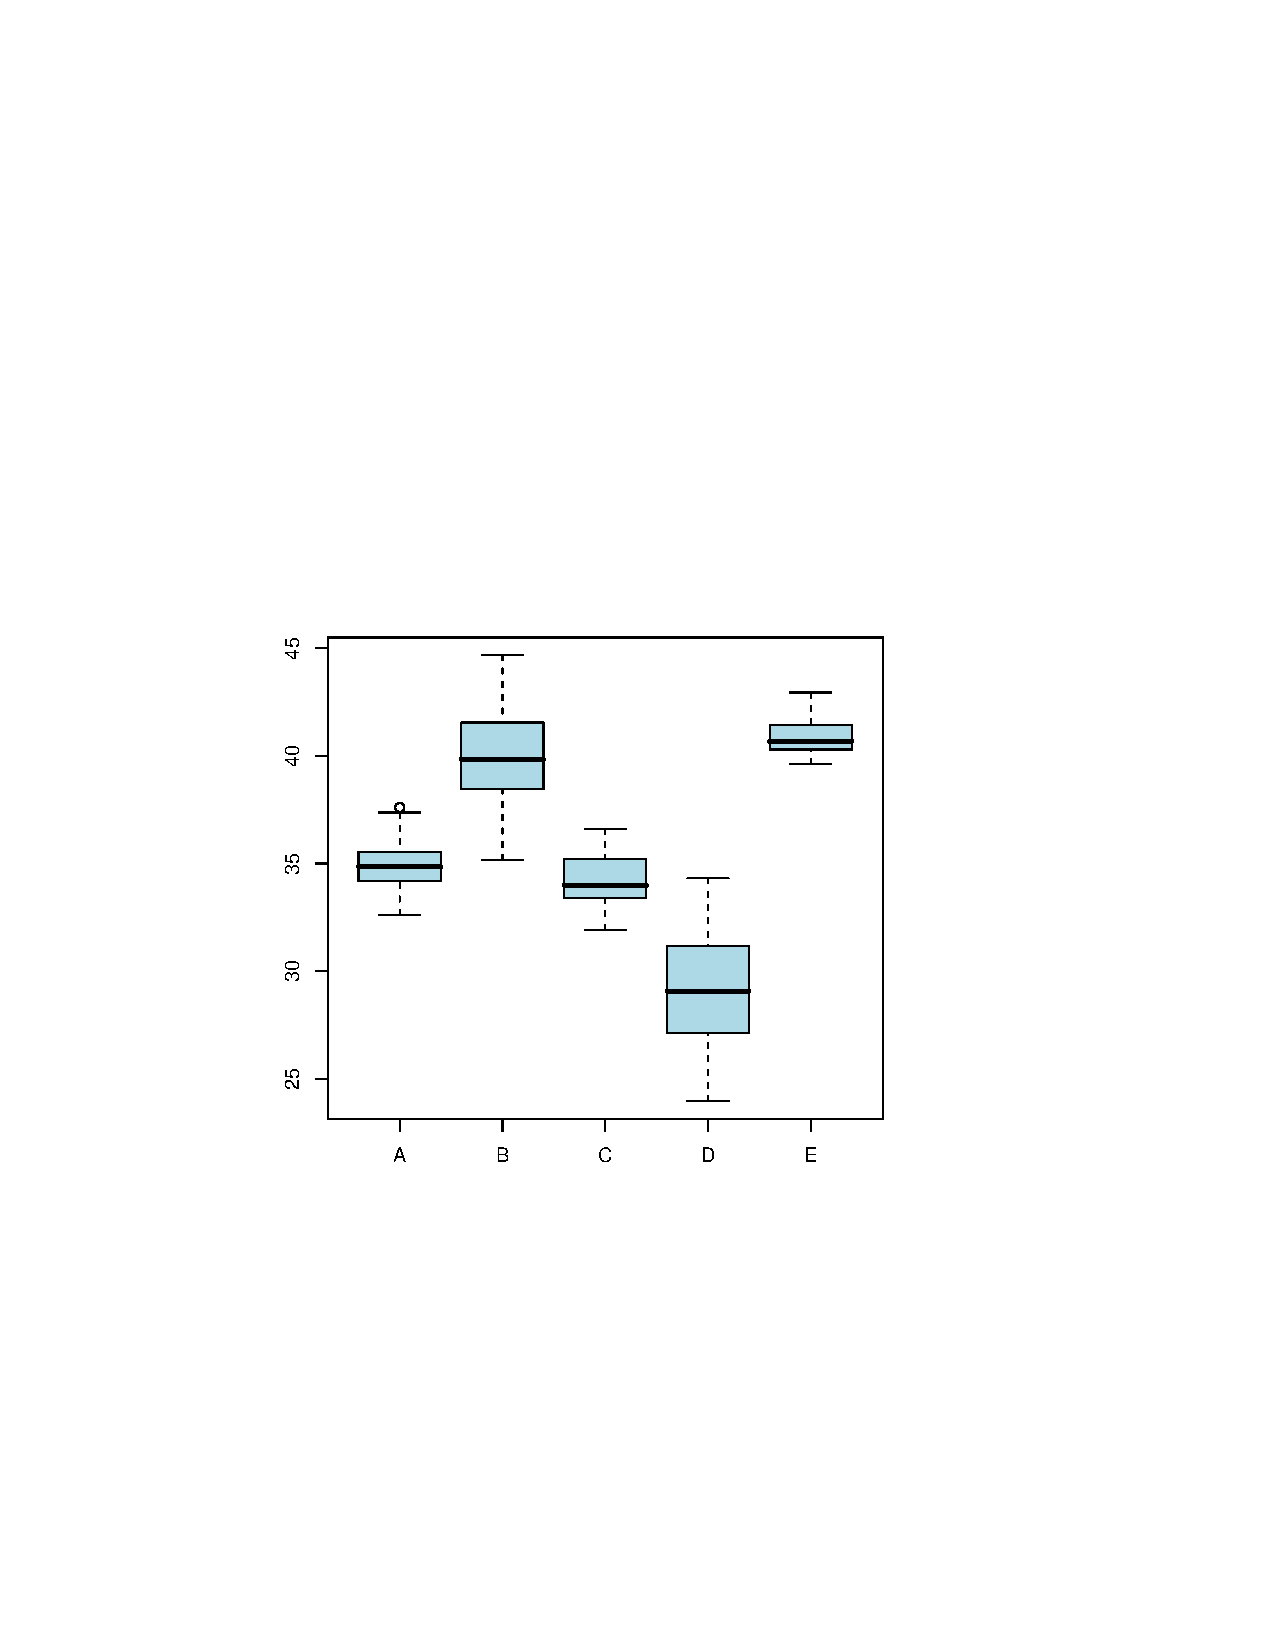
\includegraphics[width=\linewidth]{images/Diag_boite2.pdf}

    {\scriptsize Poids à la naissance (g) dans 5 populations de serpents
    (données fictives)}
    \column{0.53\textwidth}
    \small
    On veut comparer le poids à la naissance dans 5 populations de serpents.
    Que remarquez-vous?

    \medskip
    \uncover<2->{
    \begin{itemize}\itemsep 1mm
      \item Poids les plus élevés : populations \alert{B} et \alert{E}.
      \item Poids les plus faibles : population \alert{D}.
      \item Plus grande variabilité : populations \alert{B} et \alert{D}.
      \item Population A : une observation aberrante.
    \end{itemize}

    \medskip
    Comparer les moyennes de plusieurs groupes : c'est l'objet de
    l'\alert{ANOVA} (chapitre 5).
    }
  \end{columns}
\end{frame}

\begin{frame}[plain,t]
  \centerline{\LARGE\bfseries\alert{QUIZ !}}

  \medskip
  Associez chaque histogramme (A, B, C) à son diagramme en boîte (1, 2, 3).

  \medskip
  \begin{columns}[T]
    \column{0.33\textwidth}
    \centering
    \begin{tikzpicture}
      \begin{axis}[mini, width=5cm, height=3.4cm, title={A}, xticklabels={}, xmin=90, xmax=150]
        \addplot[barres] table {\tabsym};
      \end{axis}
    \end{tikzpicture}
    \column{0.33\textwidth}
    \centering
    \begin{tikzpicture}
      \begin{axis}[mini, width=5cm, height=3.4cm, title={B}, xticklabels={}, xmin=0, xmax=21]
        \addplot[barres] table {\tabdro};
      \end{axis}
    \end{tikzpicture}
    \column{0.33\textwidth}
    \centering
    \begin{tikzpicture}
      \begin{axis}[mini, width=5cm, height=3.4cm, title={C}, xticklabels={}, xmin=30.5, xmax=41]
        \addplot[barres] table {\tabgau};
      \end{axis}
    \end{tikzpicture}
  \end{columns}

  \begin{columns}[T]
    \column{0.33\textwidth}
    \centering
    \begin{tikzpicture}
      \begin{axis}[boiteh, width=5cm, height=2.6cm, title={1}, xticklabels={},
        title style={font=\scriptsize\bfseries}, xmin=30.5, xmax=41]
        \addplot[boiteprep={36.4}{38.6}{39.5}{40.2}{41}] coordinates {};
        \addplot[only marks, mark=o, mark size=1.2pt] coordinates {(30.7,1)
          (32.8,1) (33.8,1) (34.4,1) (34.5,1) (35.2,1) (35.7,1) (35.8,1)};
      \end{axis}
    \end{tikzpicture}
    \column{0.33\textwidth}
    \centering
    \begin{tikzpicture}
      \begin{axis}[boiteh, width=5cm, height=2.6cm, title={2}, xticklabels={},
        title style={font=\scriptsize\bfseries}, xmin=0, xmax=21]
        \addplot[boiteprep={0.8}{2.4}{3.8}{5.7}{10.2}] coordinates {};
        \addplot[only marks, mark=o, mark size=1.2pt] coordinates {(11.5,1)
          (13.2,1) (14.3,1) (15.3,1) (15.5,1) (17.7,1) (20,1)};
      \end{axis}
    \end{tikzpicture}
    \column{0.33\textwidth}
    \centering
    \begin{tikzpicture}
      \begin{axis}[boiteh, width=5cm, height=2.6cm, title={3}, xticklabels={},
        title style={font=\scriptsize\bfseries}, xmin=90, xmax=150]
        \addplot[boiteprep={94}{114}{121}{128}{149}] coordinates {};
      \end{axis}
    \end{tikzpicture}
  \end{columns}

  \medskip
  \uncover<2->{Pour chacune, la moyenne est-elle plus grande ou plus petite
  que la médiane?}
\end{frame}

\begin{frame}[fragile,t]{Petit détail technique : la boîte de R}
  Lorsque $n$ est \alert{pair}, la fonction \texttt{boxplot()} de R ne place
  pas les côtés de la boîte exactement en $Q_1$ et $Q_3$, mais à mi-chemin
  entre deux observations voisines (« charnières » de Tukey). Exemple avec
  12 données :
\begin{Verbatim}[fontsize=\scriptsize, formatcom=\color{TexteBoite}]
> y <- c(1, 2, 3, 7, 7, 7, 8, 9, 10, 20, 21, 24)
> quantile(y, c(0.25, 0.75))   # Q1 et Q3 (définition du cours)
 25%  75%
 6.0 12.5
> boxplot.stats(y)$stats       # bras, charnières et médiane de boxplot()
[1]  1.0  5.0  7.5 15.0 24.0
\end{Verbatim}
  Boîte de 6 à 12.5 selon la méthode du cours, de 5 à 15 dans R. Quand $n$
  est impair (serpents, tiques), les deux méthodes coïncident. En pratique,
  ces différences sont sans importance.
\end{frame}

%-------------------------------------------------------------------------------
\subsection{Complément : le diagramme quantile-quantile normal}
%-------------------------------------------------------------------------------

\begin{frame}[t]{Complément : le diagramme quantile-quantile normal}
  Plusieurs méthodes des chapitres 3 à 6 supposent que les données
  proviennent d'une \alert{loi normale} (distribution « en cloche »,
  chapitre 2). Comment le vérifier?

  \begin{itemize}\itemsep 2mm
    \item \textbf{Principe :} on compare les quantiles de l'échantillon à
      ceux auxquels on s'attendrait sous une loi normale.
    \item \textbf{Technique} (\emph{grosso modo}) : on associe à chaque
      statistique d'ordre $x_{(i)}$ le quantile de la loi normale d'ordre
      $\approx i/(n+1)$, puis on trace les $n$ points.
    \item \textbf{Lecture :} si le modèle normal est bon, les points sont
      à peu près \alert{alignés} sur une droite.
  \end{itemize}

  \medskip

  Dans R : \texttt{qqnorm(poids)}, puis \texttt{qqline(poids)} pour ajouter
  la droite de référence.

\end{frame}

\begin{frame}[t]{Exemple 1 (suite) : les serpents}
  \begin{columns}[T]
    \column{0.55\textwidth}
    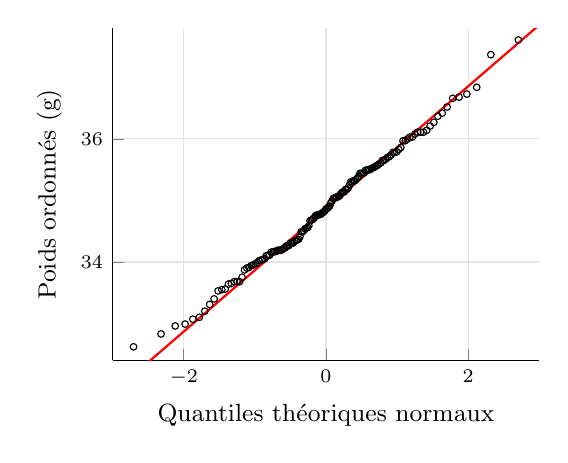
\begin{tikzpicture}
      \begin{axis}[base, width=7cm, height=5.8cm, xmin=-3, xmax=3,
        ymin=32.4, ymax=37.8, xlabel={Quantiles théoriques normaux},
        ylabel={Poids ordonnés (g)}, grid=major, grid style={black!10}]
        \addplot[red, thick, domain=-3:3] {34.8625 + 0.99705*x};
        \addplot[only marks, mark=o, mark size=1.2pt] coordinates {
(-2.706,32.62) (-2.319,32.83) (-2.120,32.96) (-1.981,32.99) (-1.872,33.07) (-1.782,33.10) (-1.704,33.20)
(-1.635,33.31) (-1.573,33.40) (-1.517,33.53) (-1.465,33.55) (-1.417,33.56) (-1.372,33.64) (-1.330,33.65)
(-1.289,33.68) (-1.251,33.68) (-1.215,33.68) (-1.180,33.75) (-1.146,33.87) (-1.114,33.90) (-1.083,33.91)
(-1.053,33.94) (-1.023,33.95) (-0.995,33.97) (-0.967,33.99) (-0.941,34.02) (-0.914,34.03) (-0.889,34.04)
(-0.864,34.05) (-0.839,34.10) (-0.815,34.11) (-0.792,34.11) (-0.769,34.16) (-0.746,34.16) (-0.723,34.17)
(-0.701,34.17) (-0.680,34.19) (-0.659,34.19) (-0.637,34.19) (-0.617,34.20) (-0.596,34.22) (-0.576,34.23)
(-0.556,34.26) (-0.536,34.26) (-0.517,34.27) (-0.497,34.31) (-0.478,34.31) (-0.459,34.31) (-0.440,34.34)
(-0.421,34.35) (-0.403,34.36) (-0.384,34.37) (-0.366,34.41) (-0.348,34.49) (-0.330,34.49) (-0.312,34.51)
(-0.294,34.54) (-0.276,34.55) (-0.259,34.56) (-0.241,34.59) (-0.224,34.67) (-0.206,34.68) (-0.189,34.69)
(-0.171,34.71) (-0.154,34.74) (-0.137,34.76) (-0.120,34.76) (-0.102,34.77) (-0.085,34.77) (-0.068,34.78)
(-0.051,34.80) (-0.034,34.81) (-0.017,34.83) (0.000,34.86) (0.017,34.87) (0.034,34.89) (0.051,34.91)
(0.068,34.96) (0.085,34.99) (0.102,35.03) (0.120,35.04) (0.137,35.05) (0.154,35.05) (0.171,35.07)
(0.189,35.07) (0.206,35.10) (0.224,35.13) (0.241,35.14) (0.259,35.14) (0.276,35.18) (0.294,35.18)
(0.312,35.20) (0.330,35.25) (0.348,35.30) (0.366,35.30) (0.384,35.32) (0.403,35.32) (0.421,35.34)
(0.440,35.36) (0.459,35.39) (0.478,35.44) (0.497,35.44) (0.517,35.44) (0.536,35.45) (0.556,35.49)
(0.576,35.49) (0.596,35.50) (0.617,35.50) (0.637,35.52) (0.659,35.53) (0.680,35.54) (0.701,35.56)
(0.723,35.57) (0.746,35.59) (0.769,35.61) (0.792,35.65) (0.815,35.65) (0.839,35.67) (0.864,35.70)
(0.889,35.71) (0.914,35.74) (0.941,35.78) (0.967,35.78) (0.995,35.79) (1.023,35.83) (1.053,35.86)
(1.083,35.97) (1.114,35.97) (1.146,36.00) (1.180,36.03) (1.215,36.03) (1.251,36.08) (1.289,36.11)
(1.330,36.11) (1.372,36.11) (1.417,36.14) (1.465,36.21) (1.517,36.27) (1.573,36.37) (1.635,36.42)
(1.704,36.52) (1.782,36.66) (1.872,36.68) (1.981,36.73) (2.120,36.84) (2.319,37.37) (2.706,37.61)
        };
      \end{axis}
    \end{tikzpicture}
    \column{0.43\textwidth}
    \small
    Les 147 points sont très bien alignés sur la droite (rouge).

    \medskip

    $\Rightarrow$ La loi normale est un modèle raisonnable pour le poids à la
    naissance de ces serpents, comme le suggérait déjà l'histogramme « en
    cloche ».

    \medskip
    Le serpent aberrant (37.61\,g) est le dernier point en haut à droite :
    à lui seul, il ne remet pas en cause le modèle.

  \end{columns}
\end{frame}

\begin{frame}[t]{Comment lire un diagramme quantile-quantile}
  \begin{columns}[T]
    \column{0.48\textwidth}
    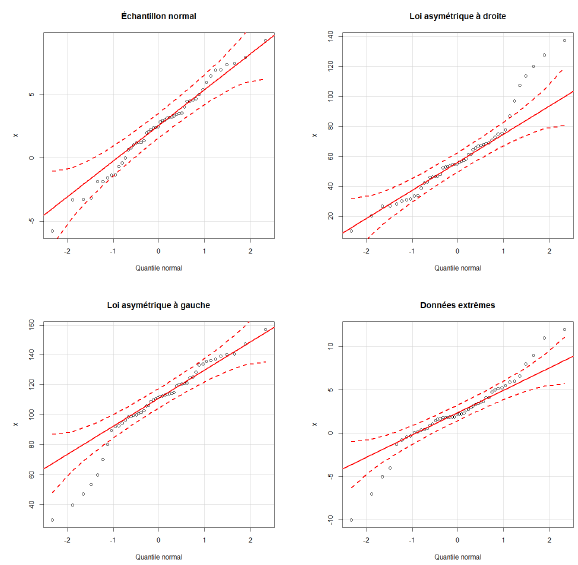
\includegraphics[width=\linewidth]{images/qqplot2.PNG}
    \column{0.5\textwidth}
    \small
    \begin{itemize}\itemsep 2mm
      \item \textbf{Échantillon normal} : points alignés (dans la bande
        pointillée).
      \item \textbf{Asymétrie à droite} : les points s'écartent vers le haut
        à droite (courbe convexe).
      \item \textbf{Asymétrie à gauche} : les points s'écartent vers le bas
        à gauche (courbe concave).
      \item \textbf{Valeurs extrêmes} (queues lourdes) : les deux extrémités
        s'écartent de la droite (forme de S).
    \end{itemize}

  \end{columns}
\end{frame}

%===============================================================================
\section[Variables qualitatives]{1.7 Diagrammes en pointes de tarte et en bâtons}
%===============================================================================

\begin{frame}[t]{Exemple 7 : une variable qualitative}
  Pour une variable \alert{qualitative}, on résume les données par un tableau
  de fréquences. On a demandé à 275 écoliers leur fruit préféré parmi les six
  fruits les plus consommés au Québec.

  \medskip
  \begin{center}
  \small
  \begin{tabular}{lccc}
    \toprule
    Fruit & Fréquence & Fréq. relative & Angle (degrés) \\
    \midrule
    Banane    & 69 & \uncover<2->{0.251} & \uncover<2->{$\frac{69}{275} \times 360 = 90.33$} \\
    Nectarine & 35 & \uncover<2->{0.127} & \uncover<2->{45.82} \\
    Orange    & 14 & \uncover<2->{0.051} & \uncover<2->{18.33} \\
    Pêche     & 39 & \uncover<2->{0.142} & \uncover<2->{51.05} \\
    Poire     & 41 & \uncover<2->{0.149} & \uncover<2->{53.67} \\
    Pomme     & 77 & \uncover<2->{0.280} & \uncover<2->{100.80} \\
    \midrule
    Total     & 275 & \uncover<2->{1} & \uncover<2->{360} \\
    \bottomrule
  \end{tabular}
  \end{center}
\end{frame}

\begin{frame}[t]{Exemple 7 (suite) : pointes de tarte et bâtons}
  \begin{columns}[T]
    \column{0.45\textwidth}
    \centering\textbf{Diagramme en pointes de tarte}

    \medskip
    \begin{tikzpicture}[scale=1.3]
      \foreach \debut/\fin/\nom/\coul in {
        0/90.33/Banane/Dominante!70,
        90.33/136.15/Nectarine/Accent!60,
        136.15/154.48/Orange/jaunelaval!70,
        154.48/205.53/Pêche/Accent!25,
        205.53/259.20/Poire/green!35,
        259.20/360/Pomme/rougelaval!45} {
        \fill[\coul, draw=white, thick] (0,0) -- (\debut:1) arc (\debut:\fin:1) -- cycle;
        \pgfmathsetmacro{\milieu}{(\debut+\fin)/2}
        \node[font=\tiny, anchor=\milieu+180] at (\milieu:1.03) {\nom};
      }
    \end{tikzpicture}

    {\scriptsize Angle (et surface) de chaque pointe $\propto$ fréquence.}
    \column{0.55\textwidth}
    \centering\textbf{Diagramme en bâtons}

    \begin{tikzpicture}
      \begin{axis}[base, width=6.8cm, height=4.6cm, ybar, bar width=0.45cm,
        ymin=0, ymax=85, ylabel={Fréquence},
        symbolic x coords={Banane,Nectarine,Orange,Pêche,Poire,Pomme},
        xtick=data, x tick label style={font=\scriptsize, rotate=30, anchor=east},
        nodes near coords, nodes near coords style={font=\tiny}]
        \addplot[fill=Dominante!60, draw=black] coordinates {(Banane,69)
          (Nectarine,35) (Orange,14) (Pêche,39) (Poire,41) (Pomme,77)};
      \end{axis}
    \end{tikzpicture}
  \end{columns}

  \medskip

  L'\oe il compare mieux des \alert{longueurs} que des \alert{angles} : le
  diagramme en bâtons est généralement plus lisible (Poire ou Pêche?).

\end{frame}

\begin{frame}[t]{Diagramme en bâtons ou histogramme?}
  \begin{itemize}\itemsep 2mm
    \item \textbf{Histogramme} : variable \alert{quantitative} continue. L'axe
      horizontal est gradué; les rectangles se touchent; c'est la
      \alert{surface} qui compte.
    \item \textbf{Diagramme en bâtons} : variable \alert{qualitative} (ou
      quantitative discrète avec peu de valeurs). Les bâtons sont séparés;
      l'ordre des catégories est arbitraire pour une variable nominale.
  \end{itemize}

  \medskip

  Dans R, pour une variable qualitative \texttt{f} :
  \texttt{table(f)} (tableau de fréquences), \texttt{barplot(table(f))}
  (bâtons), \texttt{pie(table(f))} (pointes de tarte).

  \medskip
  Les tableaux de fréquences et leur analyse (test du khi-deux) seront
  approfondis au chapitre 7.

\end{frame}

%===============================================================================
\section[Données bivariées]{1.8 Les données bivariées}
%===============================================================================

\begin{frame}[t]{Exemple 8 : deux variables à la fois}
  On mesure deux variables quantitatives $X$ et $Y$ sur chacun des $n$
  individus : les données sont $n$ couples $(x_1, y_1), \ldots, (x_n, y_n)$.

  \begin{columns}[T]
    \column{0.55\textwidth}
    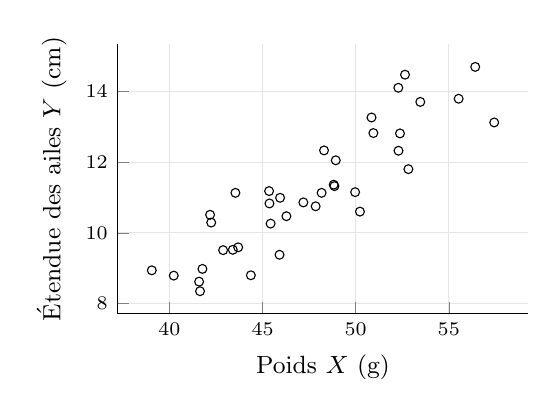
\begin{tikzpicture}
      \begin{axis}[base, width=6.8cm, height=5cm, xlabel={Poids $X$ (g)},
        ylabel={Étendue des ailes $Y$ (cm)}, grid=major, grid style={black!10}]
        \addplot[only marks, mark=o, mark size=1.6pt] coordinates {
        (52.29,14.10) (39.05,8.94) (40.23,8.79) (43.69,9.59) (50.23,10.60)
        (57.44,13.12) (42.18,10.51) (43.54,11.13) (41.59,8.62) (52.38,12.81)
        (45.35,11.18) (52.30,12.32) (45.91,9.38) (47.19,10.86) (45.94,10.99)
        (47.85,10.75) (48.82,11.36) (44.37,8.80) (46.28,10.47)
        (48.93,12.05) (48.17,11.13) (55.53,13.79) (50.85,13.26) (42.88,9.51)
        (48.86,11.32) (52.65,14.47) (45.43,10.26) (43.40,9.52) (50.95,12.82)
        (42.24,10.29) (48.30,12.33) (56.42,14.69) (49.97,11.15) (41.64,8.35)
        (52.83,11.80) (41.77,8.98) (53.47,13.70) (45.37,10.83)};
      \end{axis}
    \end{tikzpicture}
    \column{0.43\textwidth}
    \small
    Poids et étendue des ailes de 38 des 50 hirondelles de l'exemple 2 du
    chapitre 6.

    \medskip

    Ce \alert{diagramme de dispersion} (\emph{scatterplot}) montre une
    association \alert{positive} : les hirondelles plus lourdes ont tendance à
    avoir des ailes plus étendues.

    \medskip
    Dans R : \texttt{plot(x, y)}.

  \end{columns}
\end{frame}

\begin{frame}[t]{Le coefficient de corrélation}
  \begin{Boite}{Coefficient de corrélation échantillonnal}
    \[
      r = \frac{1}{n-1} \sum_{i=1}^{n}
        \left(\frac{x_i - \overline{x}}{s_x}\right)
        \left(\frac{y_i - \overline{y}}{s_y}\right)
    \]
  \end{Boite}

  \begin{itemize}\itemsep 1mm
    \item $-1 \le r \le 1$ : il mesure le degré d'association \alert{linéaire}
      entre $X$ et $Y$.
    \item $r > 0$ : association positive; $r < 0$ : association négative;
      $r \approx 0$ : pas d'association linéaire.
  \end{itemize}

  \uncover<2->{
  \textbf{Exemple 8 (suite)} : $\overline{x} = 47.53$\,g, $s_x = 4.73$\,g,
  $\overline{y} = 11.17$\,cm, $s_y = 1.74$\,cm, et \texttt{cor(x, y)} donne
  $r = \alert{0.890}$ : forte association linéaire positive.
  }
\end{frame}

\begin{frame}[t]{Quelques valeurs de $r$}
  \begin{center}
  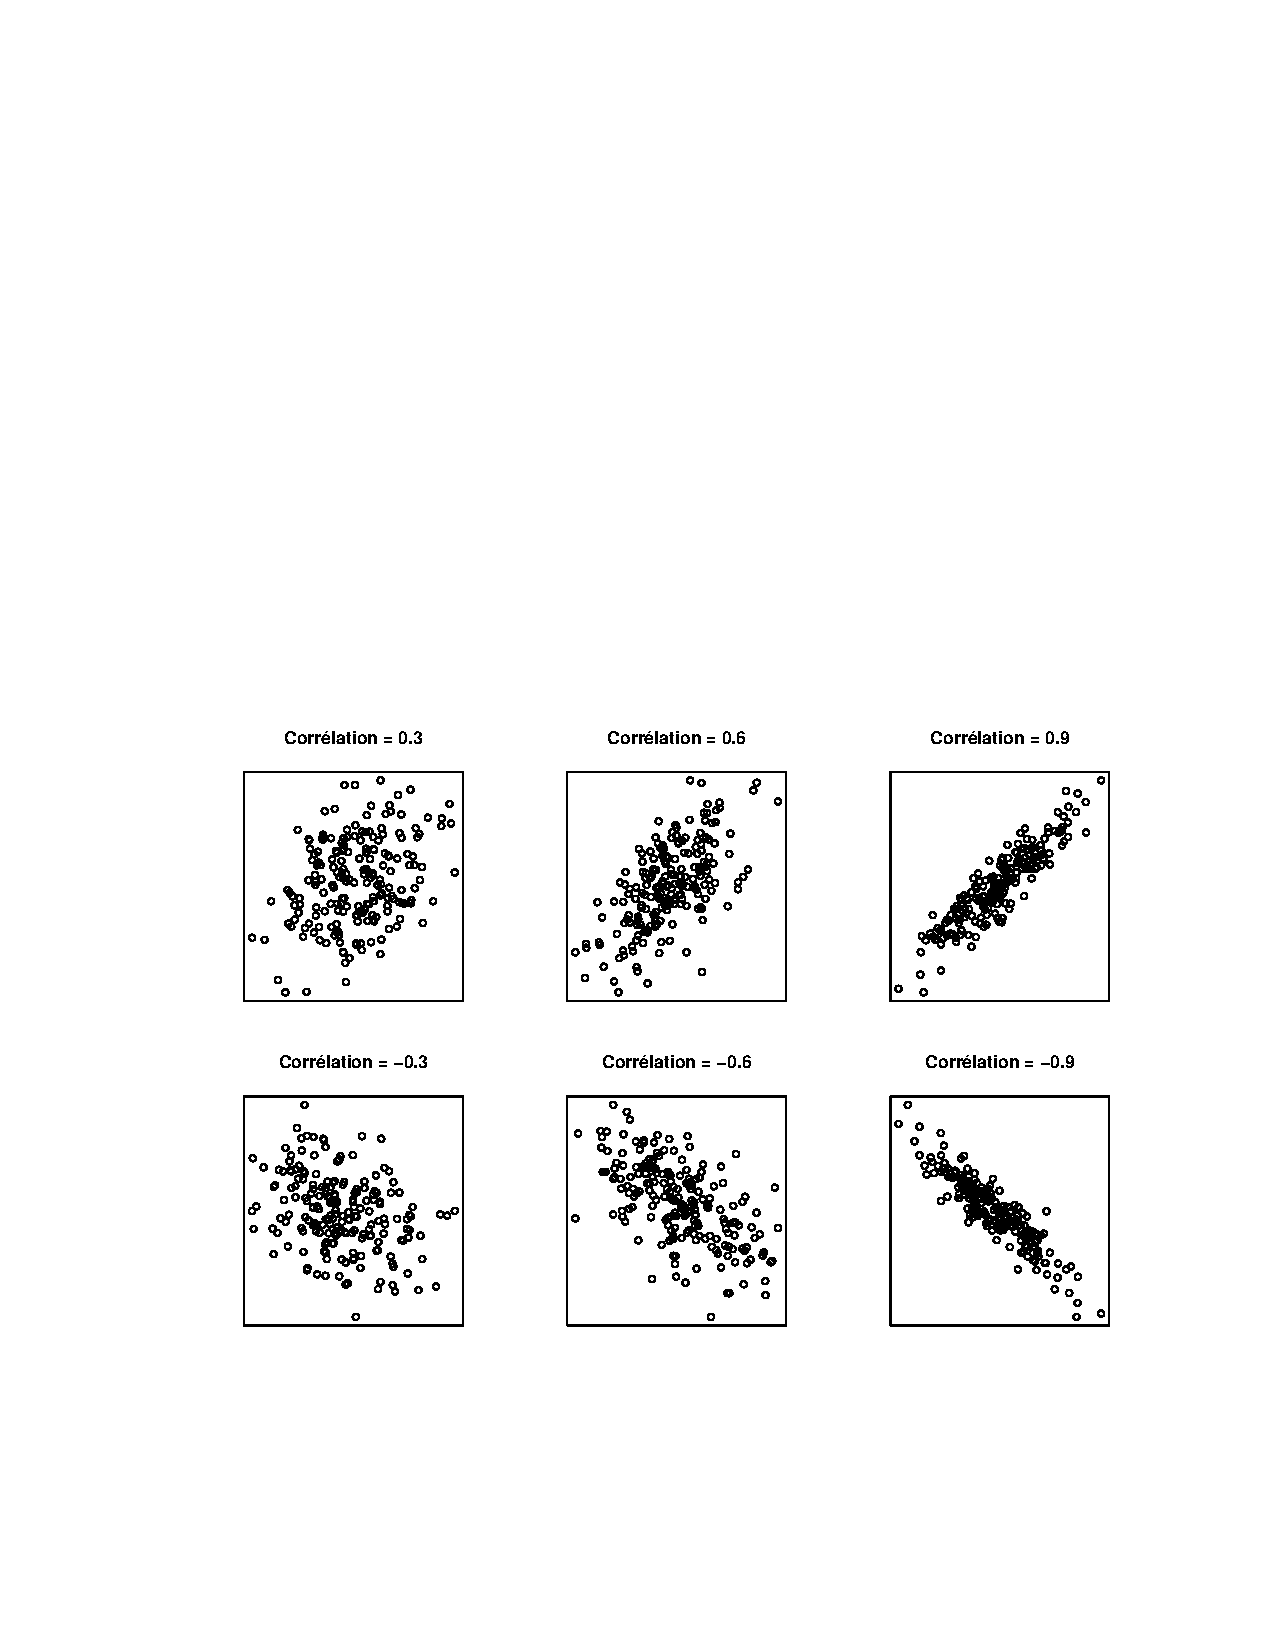
\includegraphics[width=0.52\textwidth]{images/correlations.pdf}
  \end{center}


  \small
  \textbf{Attention !} Une forte corrélation ne prouve pas une relation de
  \alert{cause à effet}. Et $r$ ne mesure que l'association \alert{linéaire} :
  une relation courbe peut donner $r \approx 0$. Toujours regarder le
  graphique! Nous y reviendrons au chapitre 6.

\end{frame}

\begin{frame}[plain,t]
  \centerline{\LARGE\bfseries\alert{QUIZ !}}

  \medskip
  Exemple 8 (hirondelles), $r = 0.890$.
  \begin{itemize}\itemsep 1.2cm
    \item On exprime maintenant le poids en kilogrammes plutôt qu'en grammes.
      La valeur de $r$ change-t-elle?
    \item<2-> On calcule plutôt la corrélation entre l'étendue des ailes et le
      poids (on inverse les rôles de $X$ et $Y$). Que vaut $r$?
  \end{itemize}
\end{frame}

%-------------------------------------------------------------------------------
% En résumé
%-------------------------------------------------------------------------------

\begin{frame}[t]{Que choisir?}
  \begin{center}
  \footnotesize
  \renewcommand{\arraystretch}{1.3}
  \begin{tabular}{p{3.4cm}p{4.4cm}p{4.6cm}}
    \toprule
    Type de données & Résumés numériques & Graphiques \\
    \midrule
    Une variable quantitative &
      $\overline{x}$, $m$, quantiles; $s$, $CV$, EIQ &
      histogramme, boîte, quantile-quantile \\
    Idem, plusieurs groupes &
      les mêmes, par groupe &
      boîtes juxtaposées \\
    Une variable qualitative &
      fréquences (relatives) &
      bâtons, pointes de tarte \\
    Deux variables quantitatives &
      coefficient de corrélation $r$ &
      diagramme de dispersion \\
    \bottomrule
  \end{tabular}
  \end{center}

  \medskip
  \textbf{À retenir :} la moyenne et l'écart-type sont sensibles aux valeurs
  extrêmes; la médiane et l'EIQ sont robustes. Toujours \alert{regarder les
  données} (graphique) avant de calculer!

  \medskip
  \textbf{Prochain chapitre :} les probabilités, pour passer de la
  description à l'inférence.
\end{frame}

\begin{frame}[fragile,t]{Aide-mémoire R}
\begin{Verbatim}[fontsize=\scriptsize, formatcom=\color{TexteBoite}]
donnees <- read.csv("serpents.csv")   # importer un fichier de données
x <- donnees$poids                    # extraire une variable
mean(x); median(x)                    # moyenne, médiane
sd(x); var(x); sd(x) / mean(x)        # écart-type, variance, CV
quantile(x, 0.4)                      # quantile d'ordre 0.4
summary(x); IQR(x)                    # résumé à cinq nombres + moyenne, EIQ
hist(x, breaks = seq(32.5, 38, by = 0.5))  # histogramme (classes choisies)
boxplot(x)                            # diagramme en boîte
boxplot(y ~ groupe, data = d)         # boîtes juxtaposées (une par groupe)
qqnorm(x); qqline(x)                  # diagramme quantile-quantile normal
table(f); barplot(table(f))           # variable qualitative f
plot(x, y); cor(x, y)                 # deux variables quantitatives
\end{Verbatim}
\end{frame}

\begin{frame}[t]{Réponses aux exemples}
  \footnotesize
  \textbf{Quiz (types de variables)} : a) qualitative nominale;
  b) quantitative continue; c) qualitative ordinale; d) quantitative discrète;
  e) quantitative continue; f) qualitative nominale; g) qualitative ordinale.

  \medskip
  \textbf{Quiz (exemple 2)} : $(45 + 35)/155 = 0.516$, soit 51.6\,\%. C'est la
  surface des rectangles au-dessus de (20, 40] :
  $10 \times 0.0290 + 10 \times 0.0226 = 0.516$. La surface totale vaut 1; la
  somme des hauteurs n'a pas d'interprétation simple.

  \medskip
  \textbf{Exemple 3} : $\overline{x} = 22$\,g, $s^2 = 6.5$\,g$^2$,
  $s = 2.55$\,g.

  \medskip
  \textbf{Quiz (moyenne, 30 patients)} : Faux en général. La moyenne reste 112
  seulement si les deux valeurs retirées ont une somme de
  $2 \times 112 = 224$.

  \medskip
  \textbf{Quiz (balance mal tarée)} : $\overline{x}$ diminue de 2\,g
  (32.882\,g); $s$ ne change pas (0.956\,g). En mg : $\overline{x} =
  32\,882$\,mg et $s = 956$\,mg (multipliés par 1000); le $CV$ ne change pas
  en passant aux mg ($0.956/32.882 = 2.9\,\%$ dans les deux unités), mais il
  avait changé lors de la correction de 2\,g (2.74\,\% $\rightarrow$
  2.91\,\%).

  \medskip
  \textbf{Exemple 5} : $q_{0.3} = 19.34$\,cm; $m = 20.4$\,cm;
  $Q_1 = x_{(2.5)} = 18.7 + 0.5 \times 0.8 = 19.1$\,cm;
  $Q_3 = x_{(5.5)} = 22.3 + 0.5 \times 2.3 = 23.45$\,cm.
\end{frame}

\begin{frame}[t]{Réponses aux exemples (suite)}
  \footnotesize
  \textbf{Quiz (médiane, 30 patients)} : Vrai. Avec $n = 30$, la médiane est
  la moyenne de $x_{(15)}$ et $x_{(16)}$; après le retrait, ces deux valeurs
  sont toujours au milieu (ce sont les 14\textsuperscript{e} et
  15\textsuperscript{e} des 28 valeurs restantes).

  \medskip
  \textbf{Quiz (séjour à l'hôpital)} : asymétrie à droite, les grandes
  valeurs tirent la moyenne vers le haut : $\overline{x} = 4.61$ jours
  $>$ $m = 3.8$ jours. Asymétrie à gauche : $\overline{x} < m$ (gestation :
  39.1 contre 39.5 semaines). Symétrique : $\overline{x} \approx m$
  (pression : 120.8 contre 121\,mmHg).

  \medskip
  \textbf{Exemple 6} : résumé à cinq nombres $(2,\ 5.5,\ 8,\ 11.5,\ 31)$;
  $\text{EIQ} = 6$; bornes $-3.5$ et 20.5; 31 est aberrante;
  $\overline{x} = 9.82$.

  \medskip
  \textbf{Quiz (histogrammes et boîtes)} : A--3, B--2, C--1.
  A : $\overline{x} \approx m$; B : $\overline{x} > m$; C : $\overline{x} < m$.

  \medskip
  \textbf{Quiz (exemple 8)} : $r$ ne change pas quand on change d'unités
  (les données sont standardisées dans la formule); il est aussi symétrique
  en $X$ et $Y$ : $r = 0.890$ dans les deux cas.
\end{frame}

%-------------------------------------------------------------------------------
\begin{frame}[t]{Références}
  Ce document est rédigé avec Beamer ainsi qu'une classe \texttt{.cls} fournie
  par Jérôme Soucy.

  \medskip
  Les diapositives sont adaptées des diapositives créées par Emmanuelle
  Reny-Nolin pour le cours STT-1920 ainsi que de celles des cours STT-1000 et
  STT-1900.

  \medskip
  Référence : C. Bélisle, \emph{STT-1920 Méthodes statistiques}, notes de
  cours, Université Laval, 2020, chapitre 1.
\end{frame}

\end{document}
